
\chapter{Numerical Results of HATDEP}

\section{Presentation}
This section presents some empirical observations à propos the new adaptive algorithm using the new introduced function $g$ defined in theorem \ref{thrm:new_g}. We hope that through the presentation of a few examples, the behaviour of the adaptive algorithm would be clearer. 

We first precise our settings, then the results and we try to give some meaningful observations and interpretations. It yields some critical ideas about how to choose the parameters. We first show how the HATDEP improves estimation in the case of windows that are too big, and secondly how the algorithm isn't harming estimations that are already good.

\section{Considered Evolution for the Parameters}
\begin{figure}
\centering
\subfloat{{
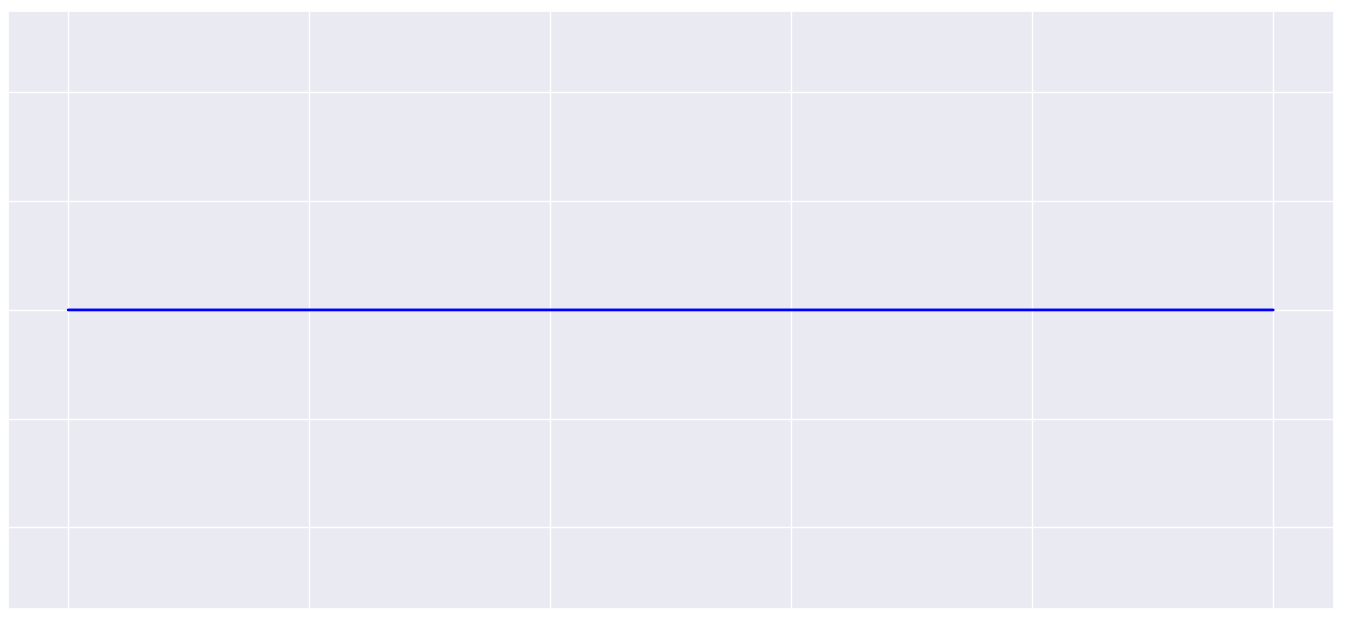
\includegraphics[width = 0.32 \textwidth]{imag/chap3/EVOL_PARAM/Figure_1.png}
}}
\subfloat{{
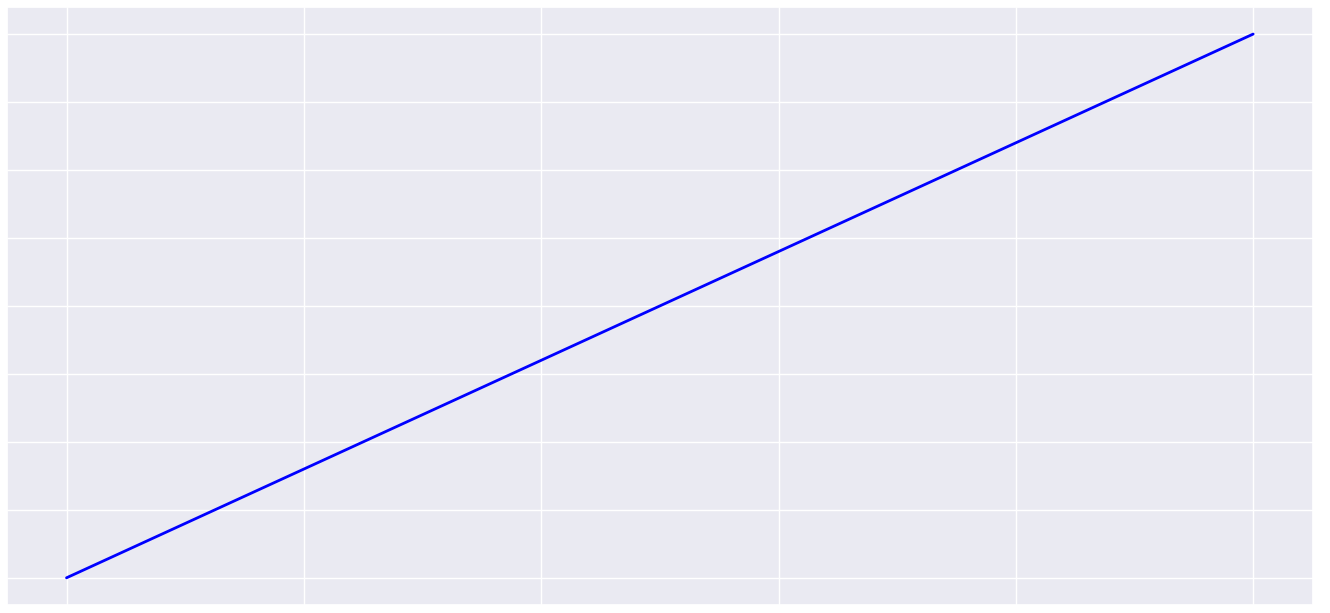
\includegraphics[width = 0.32 \textwidth]{imag/chap3/EVOL_PARAM/Figure_2.png}
}}\\
\subfloat{{
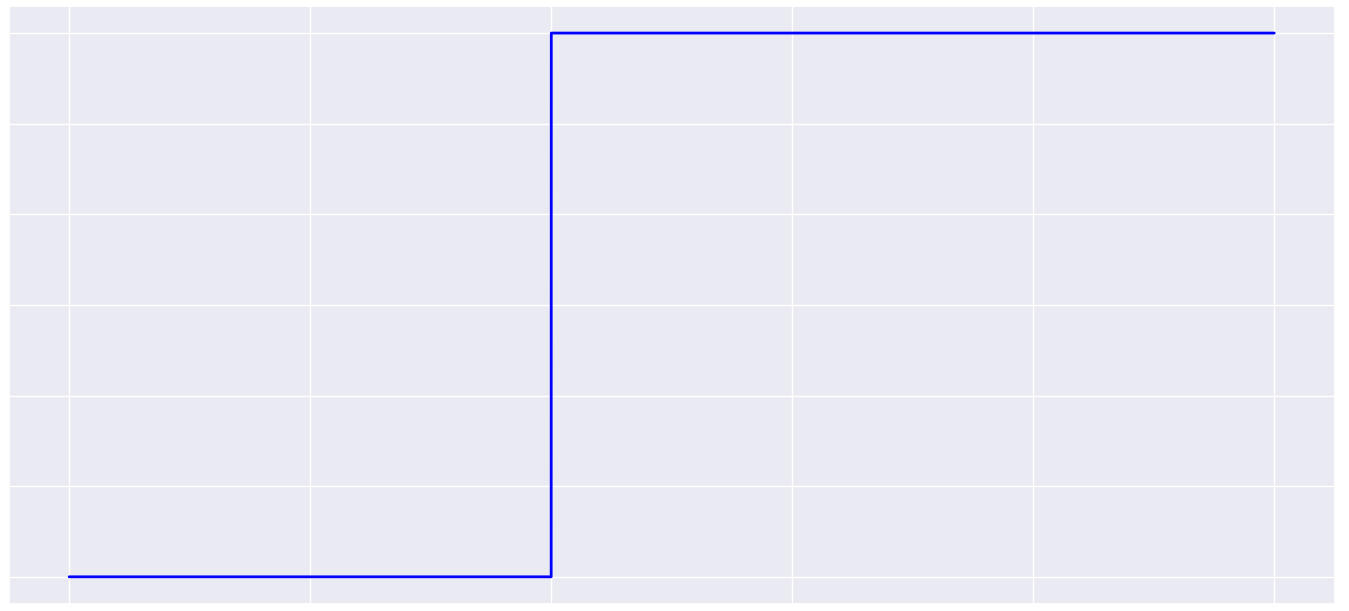
\includegraphics[width = 0.32 \textwidth]{imag/chap3/EVOL_PARAM/Figure_3.png}
}} 
\subfloat{{
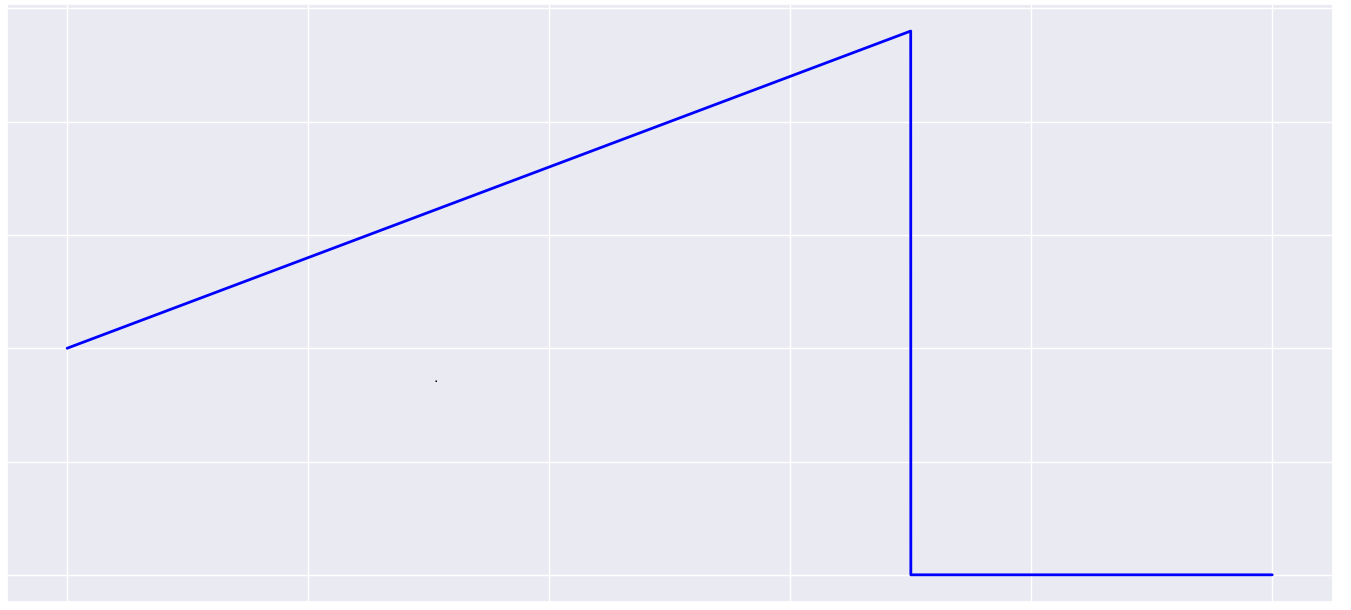
\includegraphics[width = 0.32 \textwidth]{imag/chap3/EVOL_PARAM/Figure_4.png}
}}\\
\subfloat{{
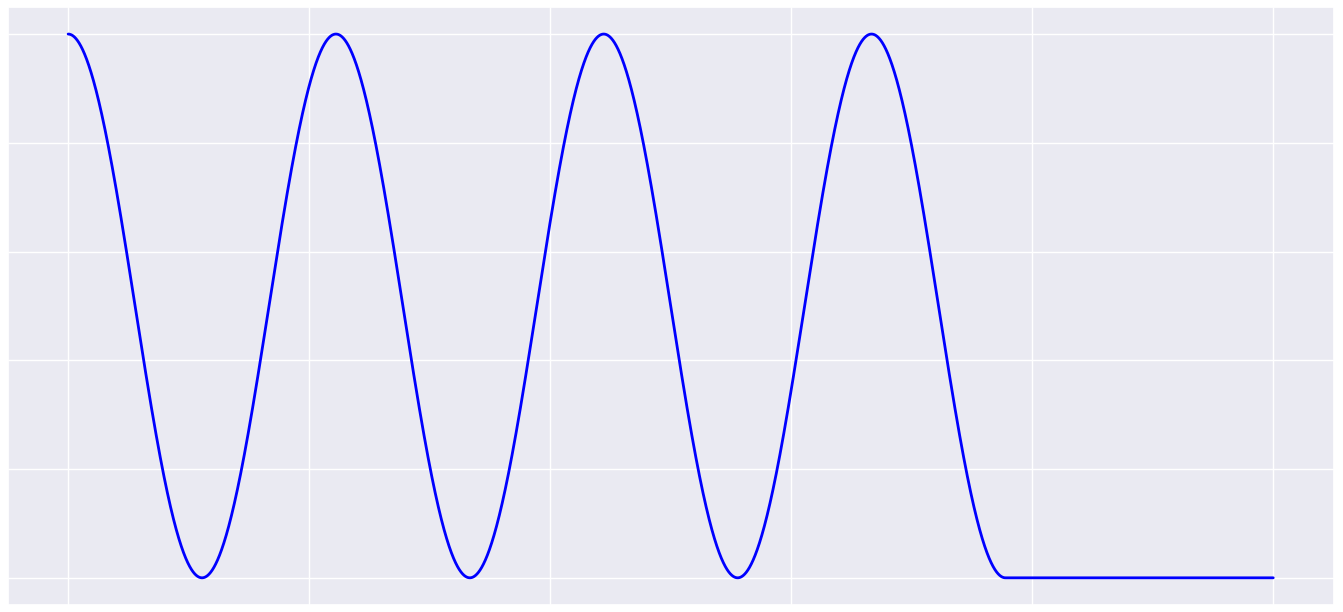
\includegraphics[width = 0.32 \textwidth]{imag/chap3/EVOL_PARAM/Figure_5.png}
}}
\caption{Plots of the different evolutions we consider for the parameters, wrt time.}
\label{fig:evol_functions}
\end{figure}

In order to consider a few different realistic situations for testing the HATDEP, we evaluate our algorithm upon a few evolution functions for the parameters. We want to see how different functions influences the results\footnote{The actual values of the functions is not important, only the shape of the evolution. Indeed, the standardization of the estimates does that only matters how the values are related to the min and the max of the function}.

We chose 

\begin{itemize}
\item constant parameters, 
\item linear evolution, 
\item one-jump evolution (piece-wise constant), 
\item linear evolution combined with one-jump evolution 
\item sinusoidal evolution followed by a constant value.
\end{itemize}

In the three last, there is a breakpoint when the function changes its behaviour: either a jump for the latter's two first, or the stop of a periodic behaviour for the latter's third function. This choice is motivated for change-point analysis in 
chapter \ref{chap:change_point}. 

We observe the basic functions in figure \ref{fig:evol_functions}.

A $M$-dimensional Hawkes process has $M+2M^2$ parameters, and for that reason, one has to choose $M+2M^2$ functions for the process. We make the choice of having the parameters $\alpha$ and $\nu$ evolving with respect to the same functions, and $\beta$ being constant. This yields 5 different cases, corresponding to the 5 different functions, and we plot in fig. \ref{fig:evol_functions_interact} how the parameters evolve with respect to each-other and to time. These coefficients are the one we use for the simulations. 

We observe the process over an interval $[0,T]$ which corresponds to roughly 7000 jumps. This number of events is quite important, and allows us to observe almost asymptotic behaviour for our estimation. At the same time, such high number of jumps is not making the simulation too long for them to not be doable. We estimated for each of the 50 points on [0.05*T,0.95 * T]\footnote{We choosed to skip the 5$\%$ at the boundaries of the simulation. That way, we hope to minimize the effect of boundaries on the estimation.}  50 times; hence each plot represents the conclusion of 2500 simulations. The data is available in CSV files available on the github of the project (cf. in appendix section \ref{csv-files}).

\begin{figure}
\centering
\subfloat{{
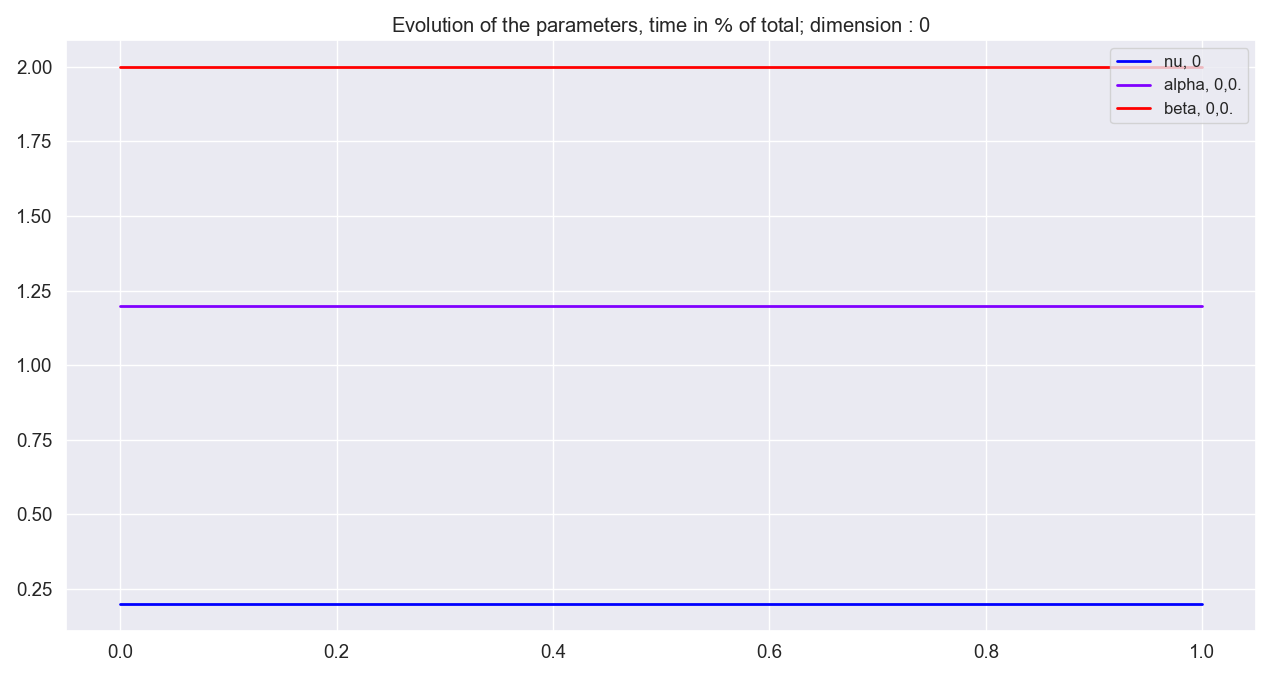
\includegraphics[width = 0.48 \textwidth]{imag/chap3/EVOL_PARAM/AFigure_1.png}
}}
\subfloat{{
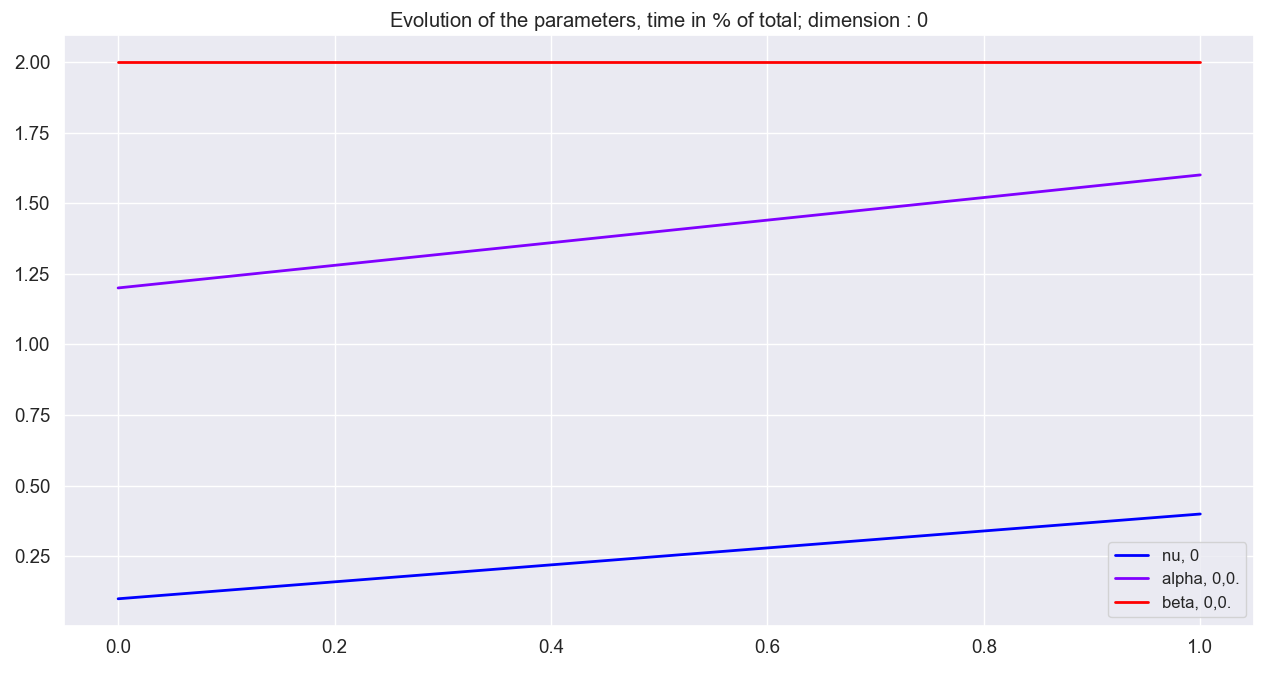
\includegraphics[width = 0.48 \textwidth]{imag/chap3/EVOL_PARAM/AFigure_2.png}
}}\\
\subfloat{{
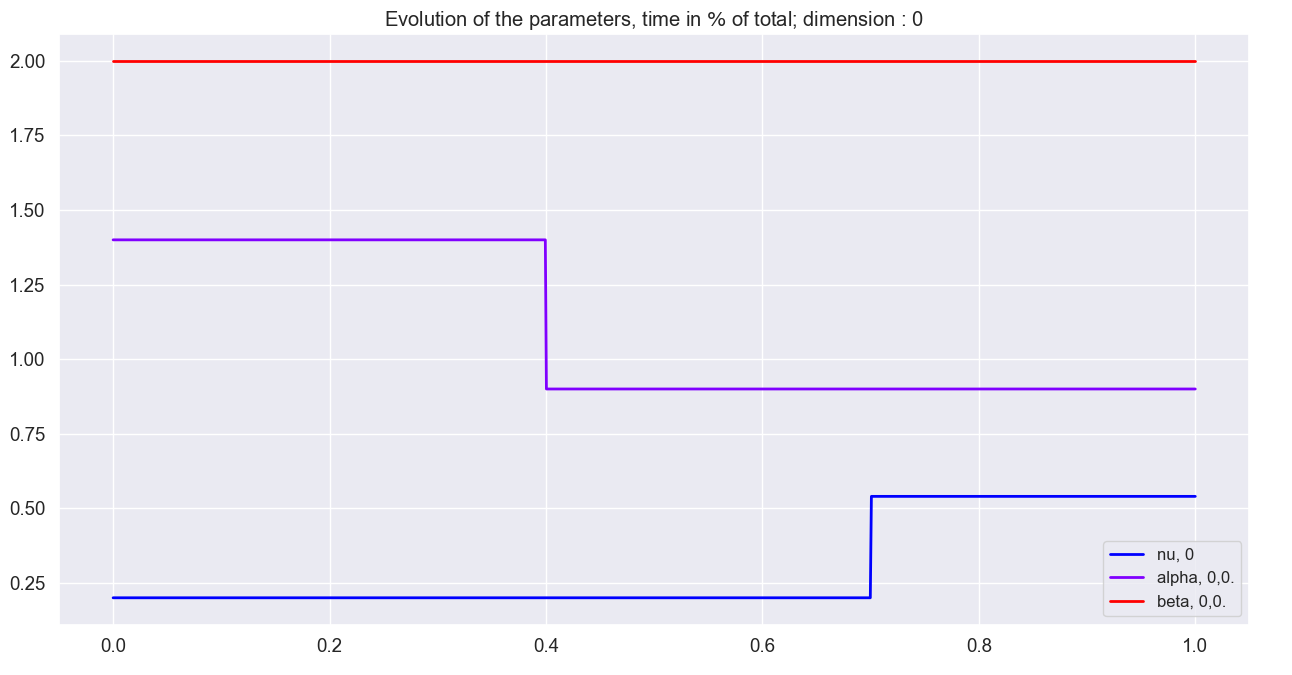
\includegraphics[width = 0.48 \textwidth]{imag/chap3/EVOL_PARAM/AFigure_3.png}
}} 
\subfloat{{
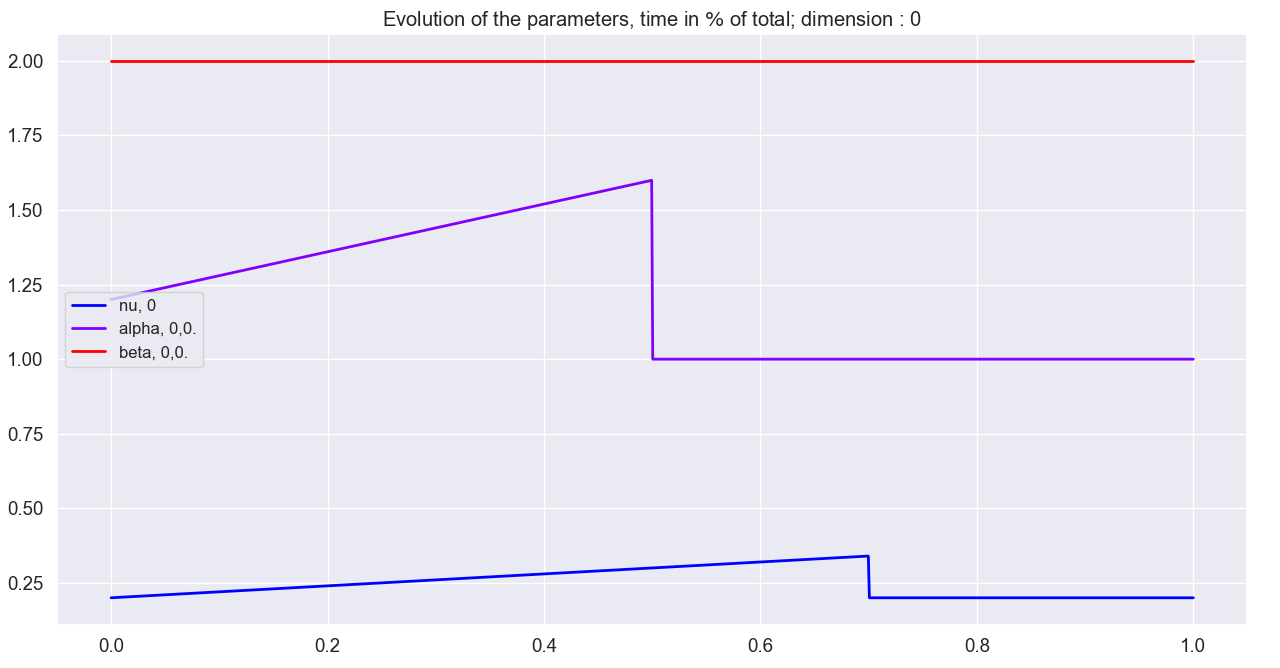
\includegraphics[width = 0.48 \textwidth]{imag/chap3/EVOL_PARAM/AFigure_4.png}
}}\\
\subfloat{{
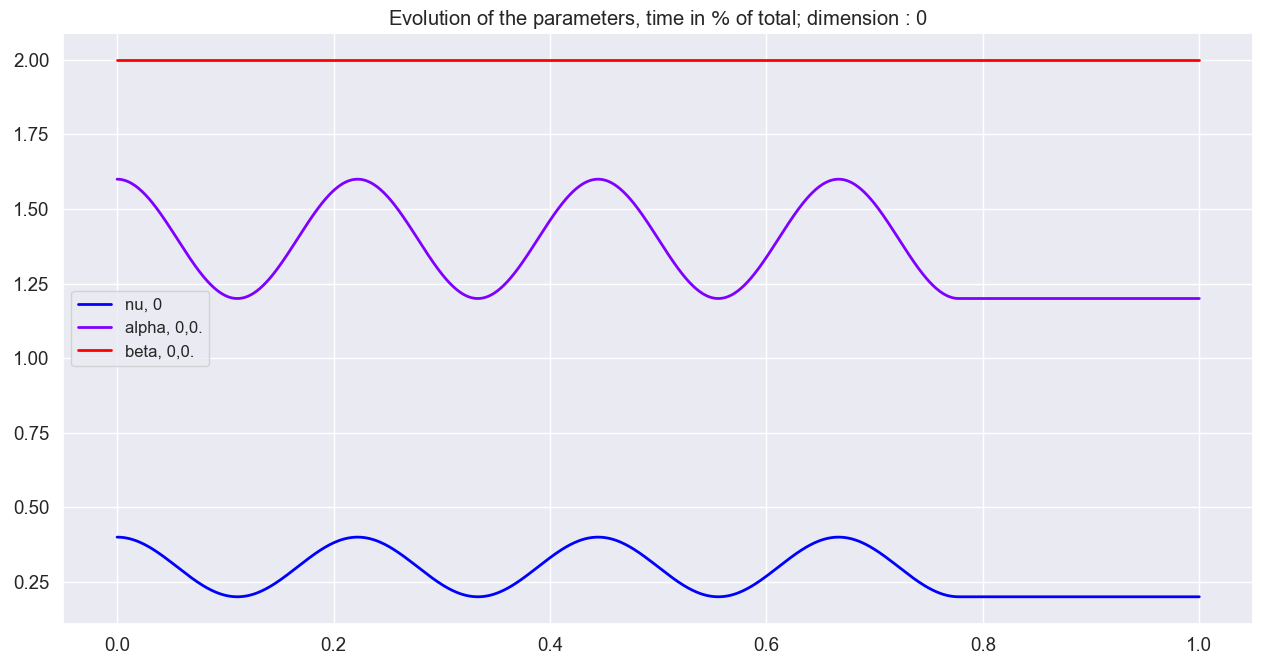
\includegraphics[width = 0.55 \textwidth]{imag/chap3/EVOL_PARAM/AFigure_5.png}
}}
\caption{Plots of the three parameters of a Hawkes process. Red is $\beta$, purple is $\alpha$ and the blue line represents the evolution of $\nu$. The 5 shapes are the one we consider and are related to the functions plotted on fig. \ref{fig:evol_functions}.}
\label{fig:evol_functions_interact}
\end{figure}













\section{HATDEP for improving performances}
\label{section_first_simul}
As a first array of trials, we consider our recommended parameters: 
\begin{itemize}
\item $L$ and $R$ defined respectively as being the $4$ and $96$ quantiles.
\item $h$ being $2.5$. We chose $l$ as a function of the first width. 
$$l = \frac{ \text{first width} }{2* \text{T max} }$$

The reason for that is that if one takes a width smaller than the total length, the kernel is not covering the whole observation window and so it is not consistent, in the sense that the criteria is global but the kernel stays local. For that reason, a good idea would be to adapt the value $l$ to the value of the original kernel. That way, one has a kernel considering all the points over the observation line, independently of its centres.
\item We are also going to use $1/3$ of the observation length as being the width for the kernels of the first estimate (hence $l = 1/6$), following the recommendation from section \ref{subsection:optimal_width} of using an arbitrary kernel width. This width is quite big relatively to the total number of jumps, and we could have used a smaller one. However, we want to observe the behaviour under non perfect condition of the adaptive algorithm.
\end{itemize}




\subsection{Constant Parameters}
The figures are drawn in appendix as: \ref{fig:first_estimate_0_alpha}, \ref{fig:first_estimate_0_beta}, \ref{fig:first_estimate_0_nu}. 


We previously mentioned how the standardization of the inputs is interfering with rescaling the kernels for constant parameters (cf. \ref{subsection:scaling}). In a few words, in such case, the scaling of the inputs is more focused on the noise rather than upon anything relevant about the data. We draw on the fig. \ref{fig:impact_g_flat} the estimation with all the respective rescaled kernels for the parameter $\nu$ (the plot is based upon the same data as for \ref{fig:first_estimate_0_nu}). 

We observe how it impacts the kernel adaptive process. The evolution is hectic and there is definitely no clear pattern. In such case, an obvious choice in order to improve the estimation is to increase the width of the kernels to the maximum and weight all the observed data in the same manner. 

In the case of constant parameters, the first estimate should parametrize the second as being a constant estimation. This case scenario is very specific and other situations are a bit more challenging.

\begin{figure}
\centering
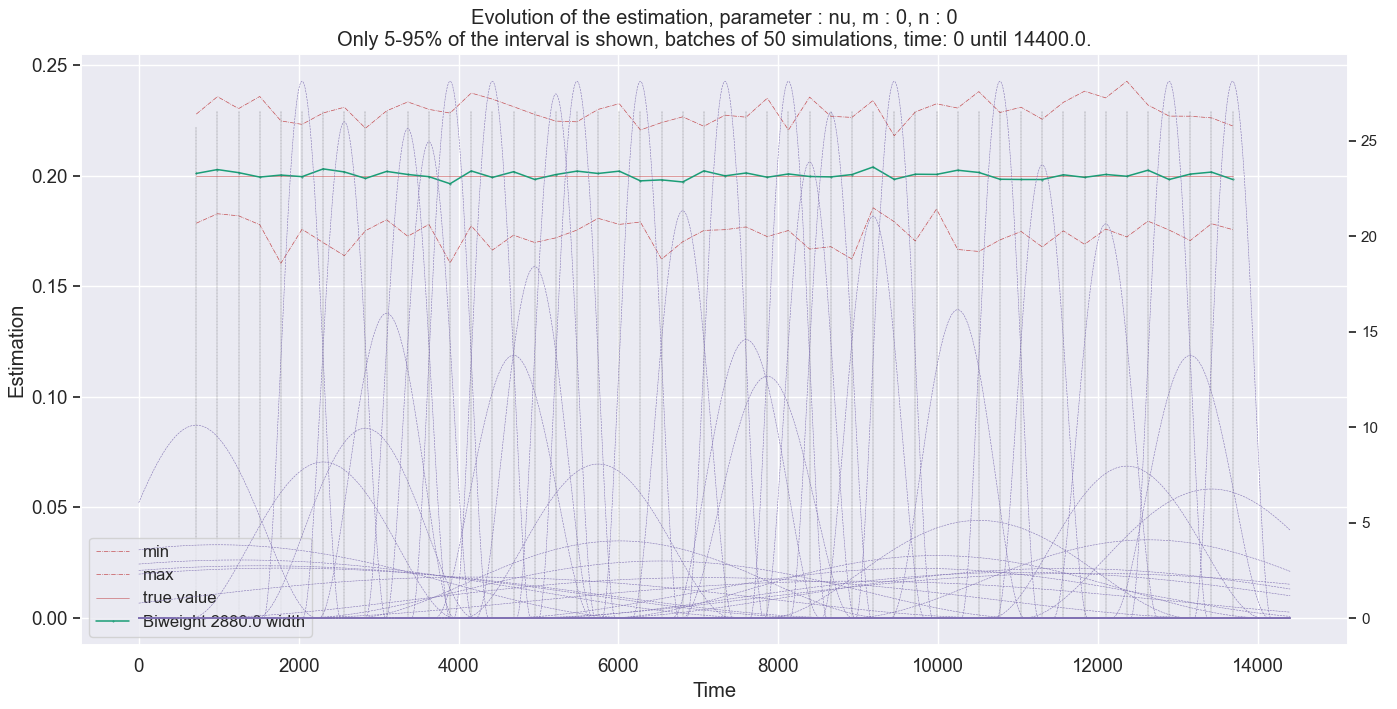
\includegraphics[width = 0.90 \textwidth]{../imag/chap3/IMPACT_G/flat_all_kernels.png}
\caption{First estimation of the parameters. We draw the kernels that are going to be used by HATDEP; this intermediary plot is useful in order to observe how different sets of first estimation influence differently the adaptive process of HATDEP. We observe that the HATDEP interpreted small variations as the extreme cases. This confirms the necessity of a threshold under which, the algorithm shouldn't consider changes as intrinsic properties and view these solely as noise.}
\label{fig:impact_g_flat}
\end{figure}


We observe an expected improvement. It isn't directly induced by $g$, but by the scaling tolerance we introduced. It deals very well with such trends. The impact of the scale on the kernels is that they became totally flat: one should be careful about the scale on the right.

\textbf{Conclusion:} Constant parameters should be treated differently than the rest. We deal with it with a tolerance threshold.




\subsection{Linear Growth}
The figures are drawn in appendix as: \ref{fig:first_estimate_1_alpha}, \ref{fig:first_estimate_1_beta}, \ref{fig:first_estimate_1_nu}.

On fig. \ref{fig:impact_g_linear}, we see the expected behaviour for the evolution of the kernels in the case of linear growth. Extreme values are estimated with smaller kernels, and values close to the mean with wider kernels\footnote{They are wide and it makes sense. Both sides compensate each-other, the parameters in the middle appear like being the average of the whole observed period.}. At the core, it is the behaviour one could expect.

\begin{figure}
\centering
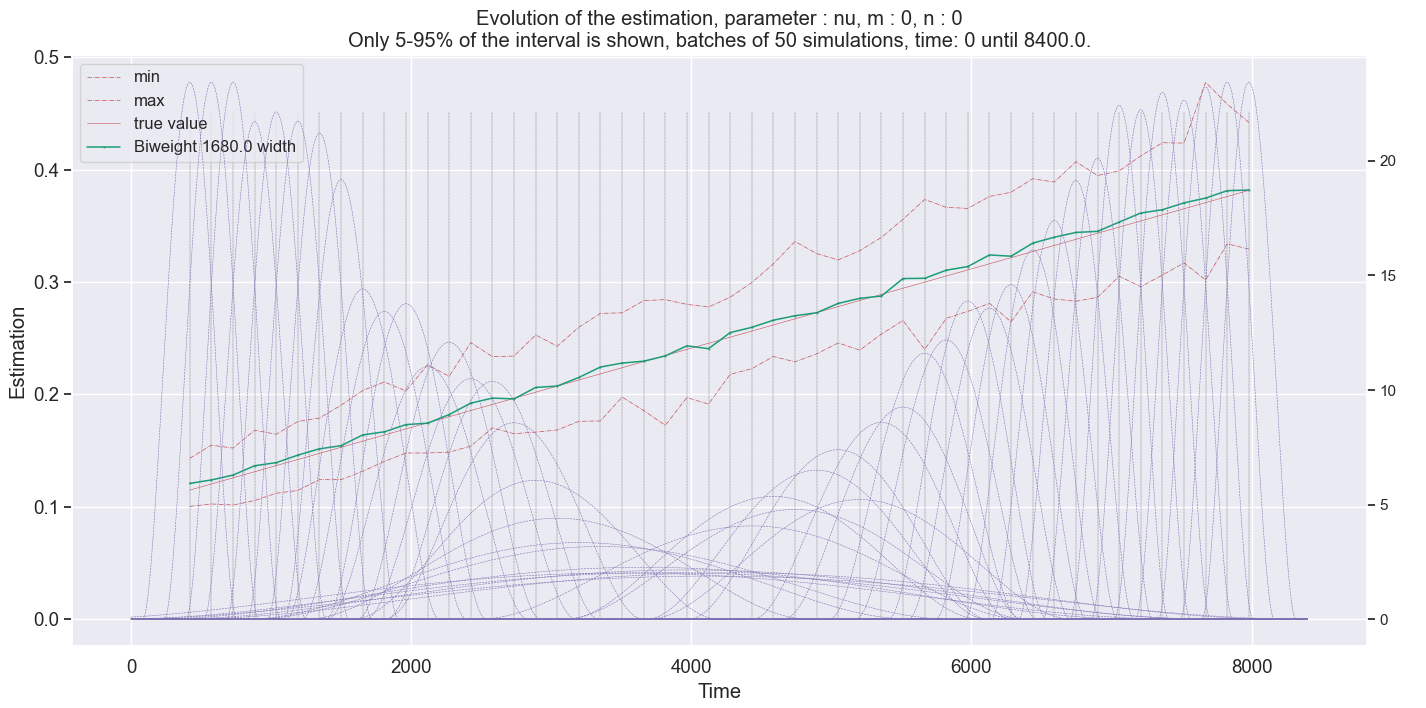
\includegraphics[width = 0.90 \textwidth]{../imag/chap3/IMPACT_G/linear_growth_all_kernels.png}
\caption{We draw the kernels that are going to be used by HATDEP with respect to the first estimate; this intermediary plot is useful in order to observe how different sets of first estimation influence differently the adaptive process of HATDEP. We observe that central estimations have wider kernels, and extreme estimations, which lie on the sides, narrower windows.}
\label{fig:impact_g_linear}
\end{figure}


\textbf{Conclusion:} Hawkes Adaptive Time Dependant Estimation of Parameters can be tried with a few different first trials, in the exact same way as KDE.




\subsection{Simple Jump}
The figures are drawn in appendix as: \ref{fig:first_estimate_2_alpha}, \ref{fig:first_estimate_2_beta}, \ref{fig:first_estimate_2_nu}.

We observe a transition phase in between the two stationary phases. It is roughly 1000 long, which is equal to half of the length of the kernel.




\begin{figure}
\centering
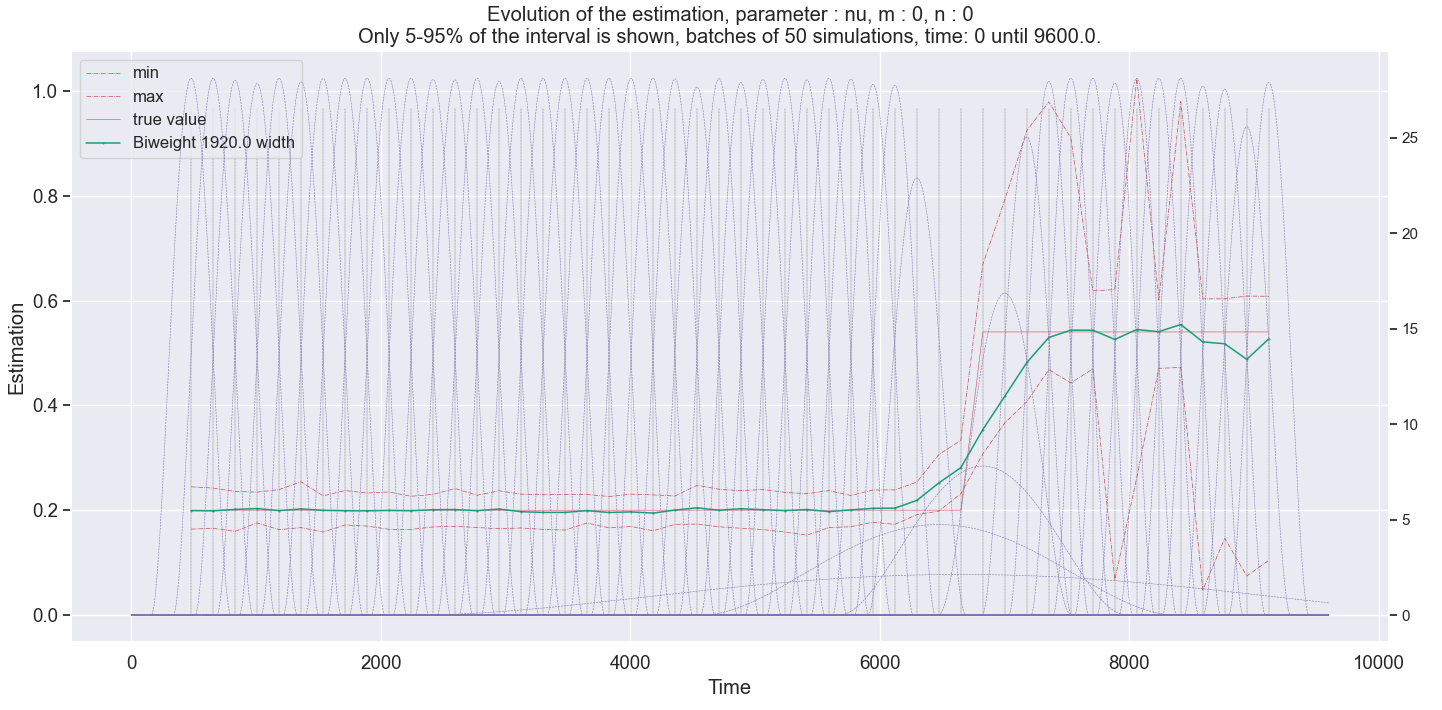
\includegraphics[width = 0.90 \textwidth]{../imag/chap3/IMPACT_G/jump_all_kernels.png}
\caption{We draw the kernels that are going to be used by HATDEP with respect to the first estimate; this intermediary plot is useful in order to observe how different sets of first estimation influence differently the adaptive process of HATDEP. We observe that the HATDEP widens the kernels in the middle of the jump but shorten the one at the end of the transition.}
\label{fig:impact_g_jump}
\end{figure}


\textbf{Conclusion:} Despite some non-expected behaviour in $\beta$'s dimension, the algorithm is doing great, reducing the transition phase of the jumps' estimation. One can however notice that the algorithm struggles to make a meaningful decision about kernel's width when the different parameters are behaving differently with respect to time. 

\begin{remarque}
The algorithm isn't adapting with respect to one parameter, but with respect to all the parameters. Since the jumps for $\alpha$ and $\nu$ are at different times, it isn't clear how to adapt in the best fashion. Overall, the two jumps are better localized, and the function is sharper (reflecting the non-continuous behaviour of it).

For the sake of comparison, we are going to show in a second approach how HATDEP captures the jump when all parameters are jumping at the same time.
\end{remarque}



\subsection{Linear Growth and Jump}
The figures are drawn in appendix as: \ref{fig:first_estimate_3_alpha}, \ref{fig:first_estimate_3_beta}, \ref{fig:first_estimate_3_nu}.

The first estimate struggles to capture accurately the jump in the parameters' function. There is a transition phase between the two behaviours which could be shortened. For parameter $\alpha$, it last for 1000, for parameter $\nu$ roughly 800. It corresponds to half the size of the kernel.

We see that the jump is better estimated after HATDEP. The transition reduces to around 600 but more importantly, one clearly distinguishes the two phases. Also, we observe that the adaptive algorithm did increase the phenomena appearing in the first graph: $\alpha$ was estimated close to $\nu$ jump (and after the adaptive process, even closer) while for nu, the jump was detected too early, and it increased with the adaptive. So, the algorithm is pinpointing some underlying phenomena, as expected. However, depending on the first estimate, the algorithm is going to do more or less good.

Another thing to consider is, in the same way as for the single jump case, that the jump isn't perfectly located, and it is a dimensionality problem. The algorithm isn't adapting with respect to one parameter, but with respect to all the parameters. Since the jumps for $\alpha$ and $\nu$ are at different times, it isn't clear how to adapt in the best fashion. Here, the algorithm has increased the kernels for all points in between the two jumps, making the left side of the jump for alpha as well as the right side of the jump for $\nu$ very precise. Overall, the two jumps are better localized, and the function is sharper (reflecting the non-continuous behaviour of it).

\textbf{Conclusion:} The algorithm is limited to low dimensional problems, like 2 or 3 dimensions maximum.

\subsection{Sinusoidal Growth}
The figures are drawn in appendix as: \ref{fig:first_estimate_4_alpha}, \ref{fig:first_estimate_4_beta}, \ref{fig:first_estimate_4_nu}.

We observe on our test image \ref{fig:impact_g_sin} that high peak values have narrow kernels and that the stationary phase after 6000 has the low narrow kernels. We expect the high points to be precise but the fact that no small kernels are left for the low points of the sinus might be an issue for a precise estimation.


The first estimate struggles to capture the variability of the sinus. The second does show some improvement: the high peaks are captured by the second estimation. However, the first estimation wasn't precise enough about the lower points of the sinus and hence the algorithm didn't precisely estimate the lowest points. A smaller first kernel would solve the problem. 


\textbf{Conclusion:} Depending on the expected behaviour of the function, whether there are many low points or many high points, one should adapt the quantiles $L$ and $R$.


\begin{figure}
\centering
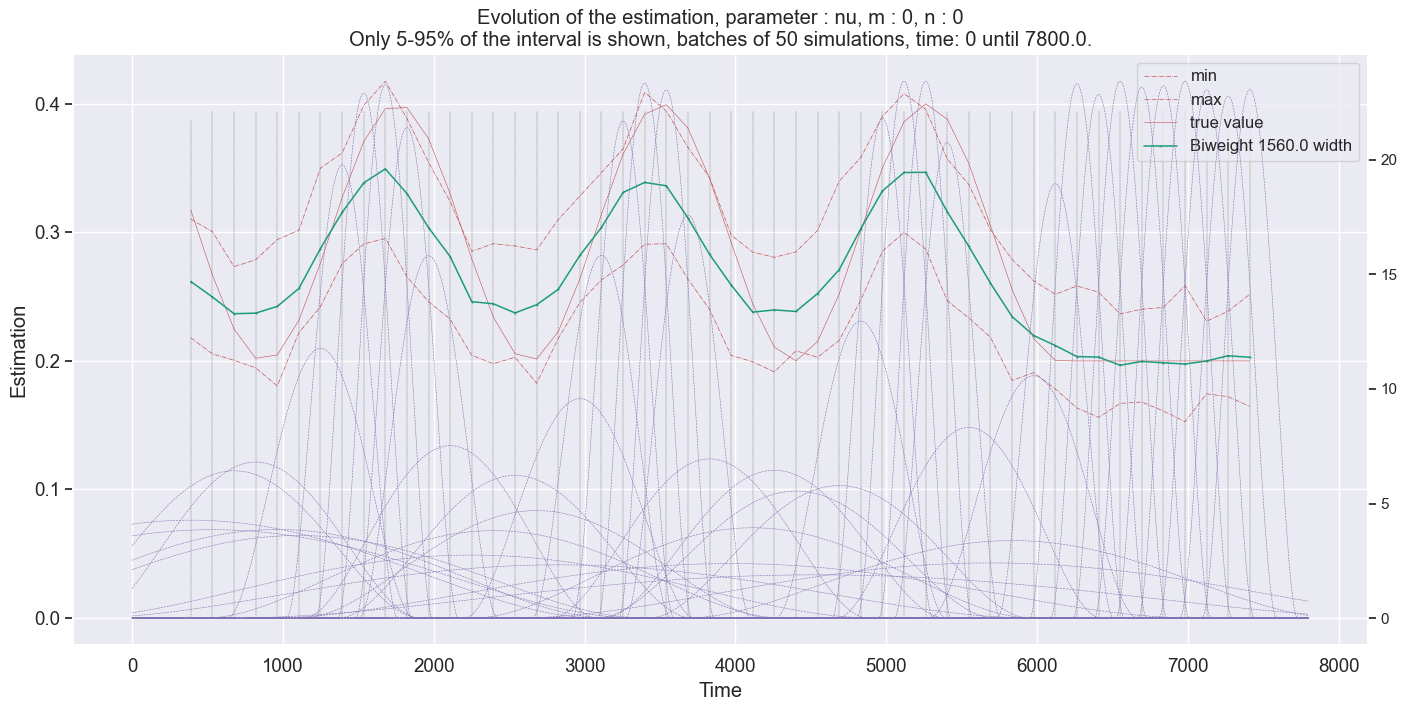
\includegraphics[width = 0.90 \textwidth]{../imag/chap3/IMPACT_G/sin_all_kernels.png}
\caption{We draw the kernels that are going to be used by HATDEP with respect to the first estimate; this intermediary plot is useful in order to observe how different sets of first estimation influence differently the adaptive process of HATDEP.}
\label{fig:impact_g_sin}
\end{figure}




\section{Better First Guess}
\label{section_second_simul}
We now use a smaller kernel from the beginning. We are studying the one jump case, the linear growth and jump case and the sinusoidal curve. For them, we use $1/5$ for all of them apart from $1/8$ for the sinusoidal curve. 



For the simple jump, the figures are drawn in appendix as: \ref{fig:second_estimate_2_alpha}, \ref{fig:second_estimate_2_beta}, \ref{fig:second_estimate_2_nu}.

For the linear growth and jump, the figures are drawn in appendix as: \ref{fig:second_estimate_3_alpha}, \ref{fig:second_estimate_3_beta}, \ref{fig:second_estimate_3_nu}.

For the sinusoidal case, the figures are drawn in appendix as: \ref{fig:second_estimate_4_alpha}, \ref{fig:second_estimate_4_beta}, \ref{fig:second_estimate_4_nu}.

In all cases, we observe that the original fit is already very good (given the precise windows) and the HATDEP doesn't harm the estimation by adjusting the windows. It also improves the interesting parts, as the extreme parts of the sinus, or the discontinuity in the jump case.


We also give a closer look at the case where all the jumps are at the same time. We had to change the parameters for HATDEP a bit, but the results are astonishingly good. The figures are drawn in appendix as: \ref{fig:second_estimate_12_alpha}, \ref{fig:second_estimate_12_beta}, \ref{fig:second_estimate_12_nu}.




\section{Conclusion About the Algorithm}
HATDEP is a two-step adaptive algorithm, inspired by the theory of Kernel Density Estimation, used in order to get more precise results in the MSE sense of the estimation of time-dependant Hawkes process' parameters. It relies upon the idea that extreme points estimated should have narrower kernels. Based on that idea, we created a HATDEP function out of two sinuses. We tested HATDEP for a few situations, and it showed significant improvements. It reduces the interval over which the discontinuities are captured by a transition effect, and short time effects (like peaks) are also more visible.

It suffers nonetheless from a problem of dimensionality. Better results are given by processes with similar behaviour on every dimension.

We recommand a flexible choice of parameters, though each evolution of parameters is unique and should be handled differently at the essence. For that reason, we recommand that one checks first how the kernels look like on a first plot (like on the plot \ref{fig:essential_check_triple}) in order to know if the algorithm tailored the kernels to our will.

\begin{figure}
\centering
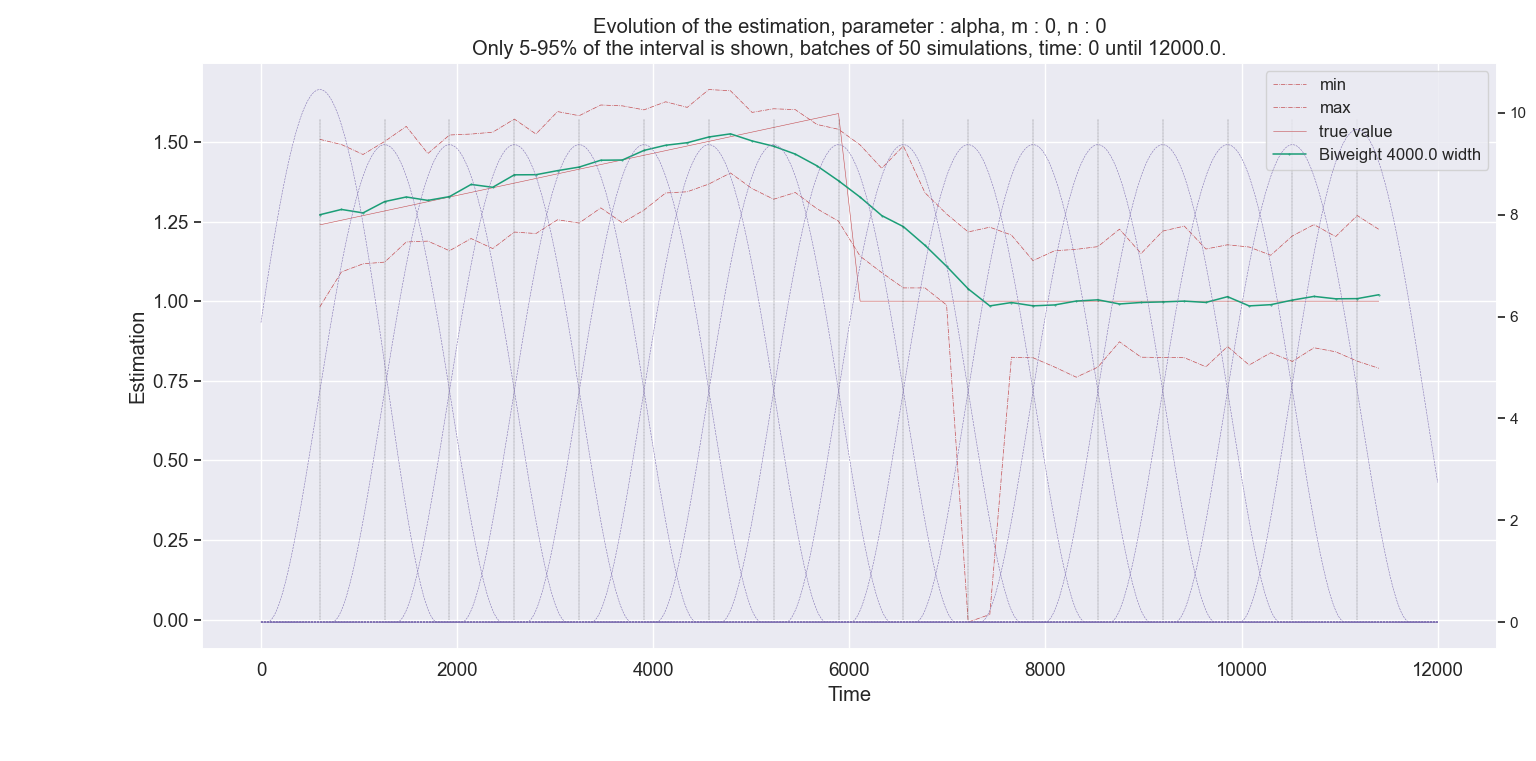
\includegraphics[width = 0.90 \textwidth]{../imag/chap3/triple/Figure_2.png}
\caption{Presentation of the adaptive kernels for the case all jumps at the same time. Relative width of a kernel : $1/3$, $L = 0.04$, $R = 0.9$, $l = 0.9$, $h = 2.5$. Data in \protect \path{second_estimations/super_smaller_12_first.csv}.}
\label{fig:essential_check_triple}
\end{figure}
